\documentclass[11pt, a4paper]{article}

%\usepackage[T1]{fontenc}
%\usepackage{fullpage}

\usepackage[utf8]{inputenc} % comment when using lualatex
\usepackage[italian]{babel} % lingua e a-capo-sillabato
\usepackage{graphicx}
\usepackage[hidelinks]{hyperref,xcolor} % link di pagina
\usepackage[bottom]{footmisc} % note appiccicate al fondo della pagina
\usepackage{float} % per posizionamento immagini
\usepackage{amsthm}
\usepackage{fancyhdr}
\usepackage[font=small,labelfont=bf]{caption} % small font for caption (and bold Figure word)

\pagestyle{fancy}
\fancyhf{}% Clear header/footer
\fancyfoot[C]{\thepage} %add page number
\fancyhead[C]{\footnotesize\textit{Documento:} D4 \hfill SleepCode \hfill \textit{Versione:} 1.0}
\renewcommand{\headrule}{{\color{red!70}\rule{\textwidth}{2pt}}}
\setlength{\headheight}{22pt}
\hypersetup{
    colorlinks=true,
    linkcolor=cyan,
    filecolor=magenta,      
    urlcolor=blue,
    }

%\pagestyle{myheadings}
%\markright{John Smith\hfill On page styles\hfill}

\renewcommand\UrlFont{\color{blue}\rmfamily}

\theoremstyle{definition}

\newtheorem{funcreq}{RF} %% numerazione dei requisiti funzionali
\newtheorem{nonfuncreq}{RNF} %% requisiti non funzionali
\newtheorem{backend}{BE}
\newtheorem{frontend}{FE}

\title{Documento di Sviluppo}

\author{Raffaele \textsc{Castagna}\\
Alberto \textsc{Rovesti}\\
Zeno \textsc{Saletti}}

\newcommand{\groupNumber}{G17}


% —

% Web address for the project (if any)
% \newcommand{\homepage}{\url{https://www.}}

% data
\date{\today}

\makeatletter{}


\newcommand\blfootnote[1]{%
  \begingroup
  \renewcommand\thefootnote{}\footnote{#1}%
  \addtocounter{footnote}{-1}%
  \endgroup
}

% IL PREAMBOLO FINISCE QUI %%%%%%%%%%%%%%%%%%%%%%%%%%%%%%%%%%%%%%%%%%%%%%%%%%%%






\begin{document}

% La pagina di copertina si trova in un file .tex a parte
% NON MODIFICARE QUESTO COMANDO!!!
\begin{titlepage}
\newcommand{\HRule}{\rule{\linewidth}{0.3mm}} % Defines a new command for horizontal lines, change thickness here
\center % Centre everything on the page

%------------------------------------------------
%	Logo
%------------------------------------------------

\includegraphics[width=0.3\textwidth]{materiale/UniTrento_logo_ITA_colore.png}\\[0.5cm]
%------------------------------------------------
%	Headings
%------------------------------------------------
\textsc{\Large Dipartimento di Ingegneria\\e Scienza dell'Informazione}\\[1.5cm]

{\Huge\textbf{Sleep Code}}\\[0.5cm]
\textsc{\large Progetto per il Corso di Ingegneria del Software}\\
\textsc{\large Anno Accademico 2023-2024}\\[0.5cm]

%------------------------------------------------
%	Title
%------------------------------------------------

\HRule\\[0.4cm]
{\huge\bfseries \@title}\\[0.1cm]
\HRule\\[1cm]

\begin{minipage}{\textwidth}
\begin{flushleft}
\textit{Descrizione:} documento di analisi dei requisiti funzionali, non funzionali, front-end e back-end.
\end{flushleft}
\end{minipage}\\[1.5cm]


\begin{minipage}{0.4\textwidth}
\begin{flushleft}
\large
\textit{Numero documento:} D1
\end{flushleft}
\end{minipage}
\begin{minipage}{0.4\textwidth}
\begin{flushright}
\large
\textit{Versione documento:} 2.4
\end{flushright}
\end{minipage}\\[1.5cm]

%------------------------------------------------
%	Author(s)
%------------------------------------------------
\begin{minipage}{0.4\textwidth}
\begin{flushleft}
\large
\textit{Membri del gruppo:}\\
\@author % Your name
\end{flushleft}
\end{minipage}
~
\begin{minipage}{0.4\textwidth}
\begin{flushright}
\large
\textit{Numero gruppo: }
\groupNumber
\end{flushright}
\end{minipage}

% 	If you don't want a supervisor, uncomment the two lines below and comment the code above
% 	{\large\textit{Author(s)}}\\
% 	\@author % Your name

%------------------------------------------------
%	Date
%------------------------------------------------

\vfill\vfill
\textit{Ultima revisione:}
{\@date}

\end{titlepage}

\tableofcontents\blfootnote{\textbf{Consigli utili per la consultazione del testo:} Se il lettore per file \texttt{.pdf} attualmente in uso lo consente, è possible navigare con più semplicità e velocità all'interno di questo documento cliccando sugli elementi dell'indice.}


\newpage
\section{Scopo del documento}
Il presente documento riporta tutte le informazioni richieste e necessarie per lo Sviluppo
di una parte dell'applicazione Sleepcode.
In particolare, presenta:
\begin{itemize}
  \item User Flow legato al ruolo dell'utente (amministratore,autenticato e non)
  \item User Flow legato all'uso del sito
  \item Documentazione delle Api attraverso API Model e Modello delle risorse
  \item Api Fornite per interagire con l'applicazione
  \item Descrizione delle api fornite
  \item Risultati delle test suite applicata sulle api
\end{itemize}


\newpage
\section{User Flows}
In questa sezione del documento di sviluppo vengono riportati gli user Flows. Lo scopo degli User Flows
è quello di poter specificare le azioni disponibili all'utente e le conseguenza di esse. Sono stati individuati 2 tipi di User flow, uno per 
tutto ciò che riguarda l'autenticazione e il profilo utente, e un'altro che riguarda le azioni disponibili ai diversi ruoli di utente.
Teniamo a ricordare che tutte le immagini sono disponibili ad alta risoluzione nell'appropriata cartella del D4.
Di seguito esponiamo la legenda per i simboli utilizzati
\\
\\
\begin{center}
  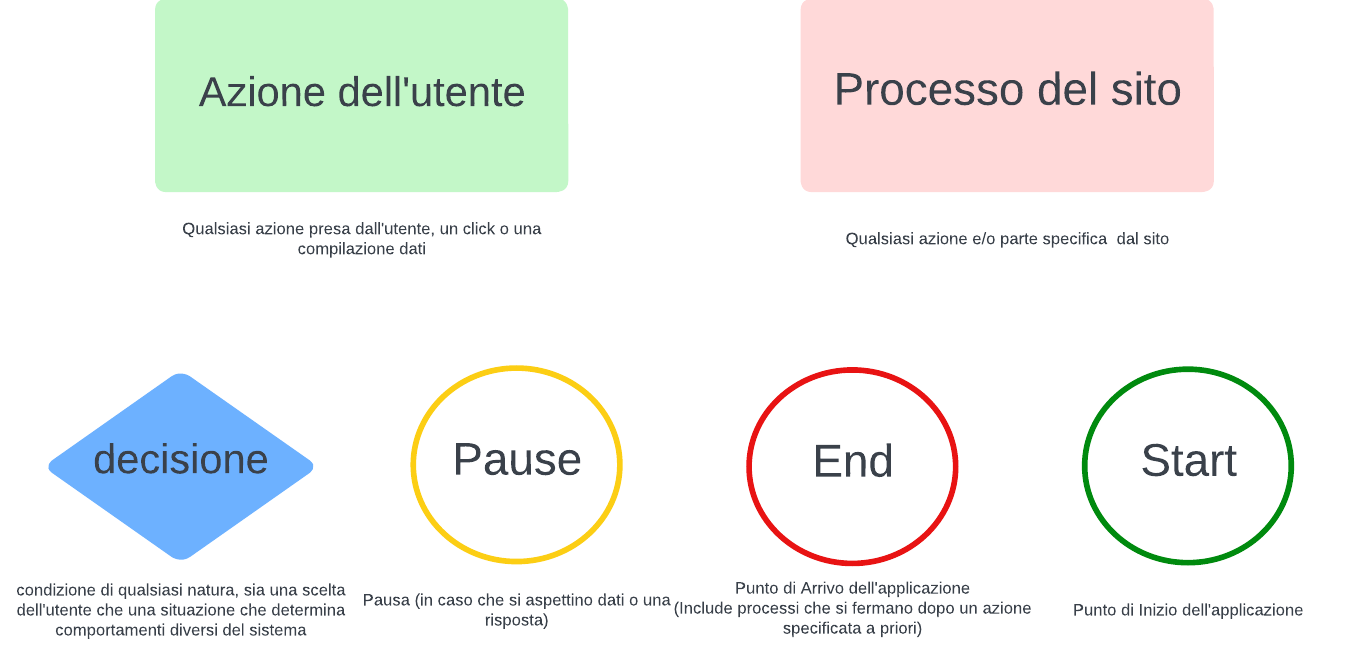
\includegraphics{materiale/UserFlow Symbols.png}
\end{center}
\newpage
\subsection{Azioni riguardanti l'autenticazione}
Questo User Flow è specifico per tutte le azioni che riguardo l'autenticazion e ciò che fa parte di essa. Si ricorda che in ogni momento della navigazione
l'utente è in grado di poter autenticarsi,tornare alla home e al catalogo tramite una apposita Navbar che è presente in ogni pagina del sito web. Parte di queste interazioni sono state rimosse per
rendere l'User Flow pià leggibile.
  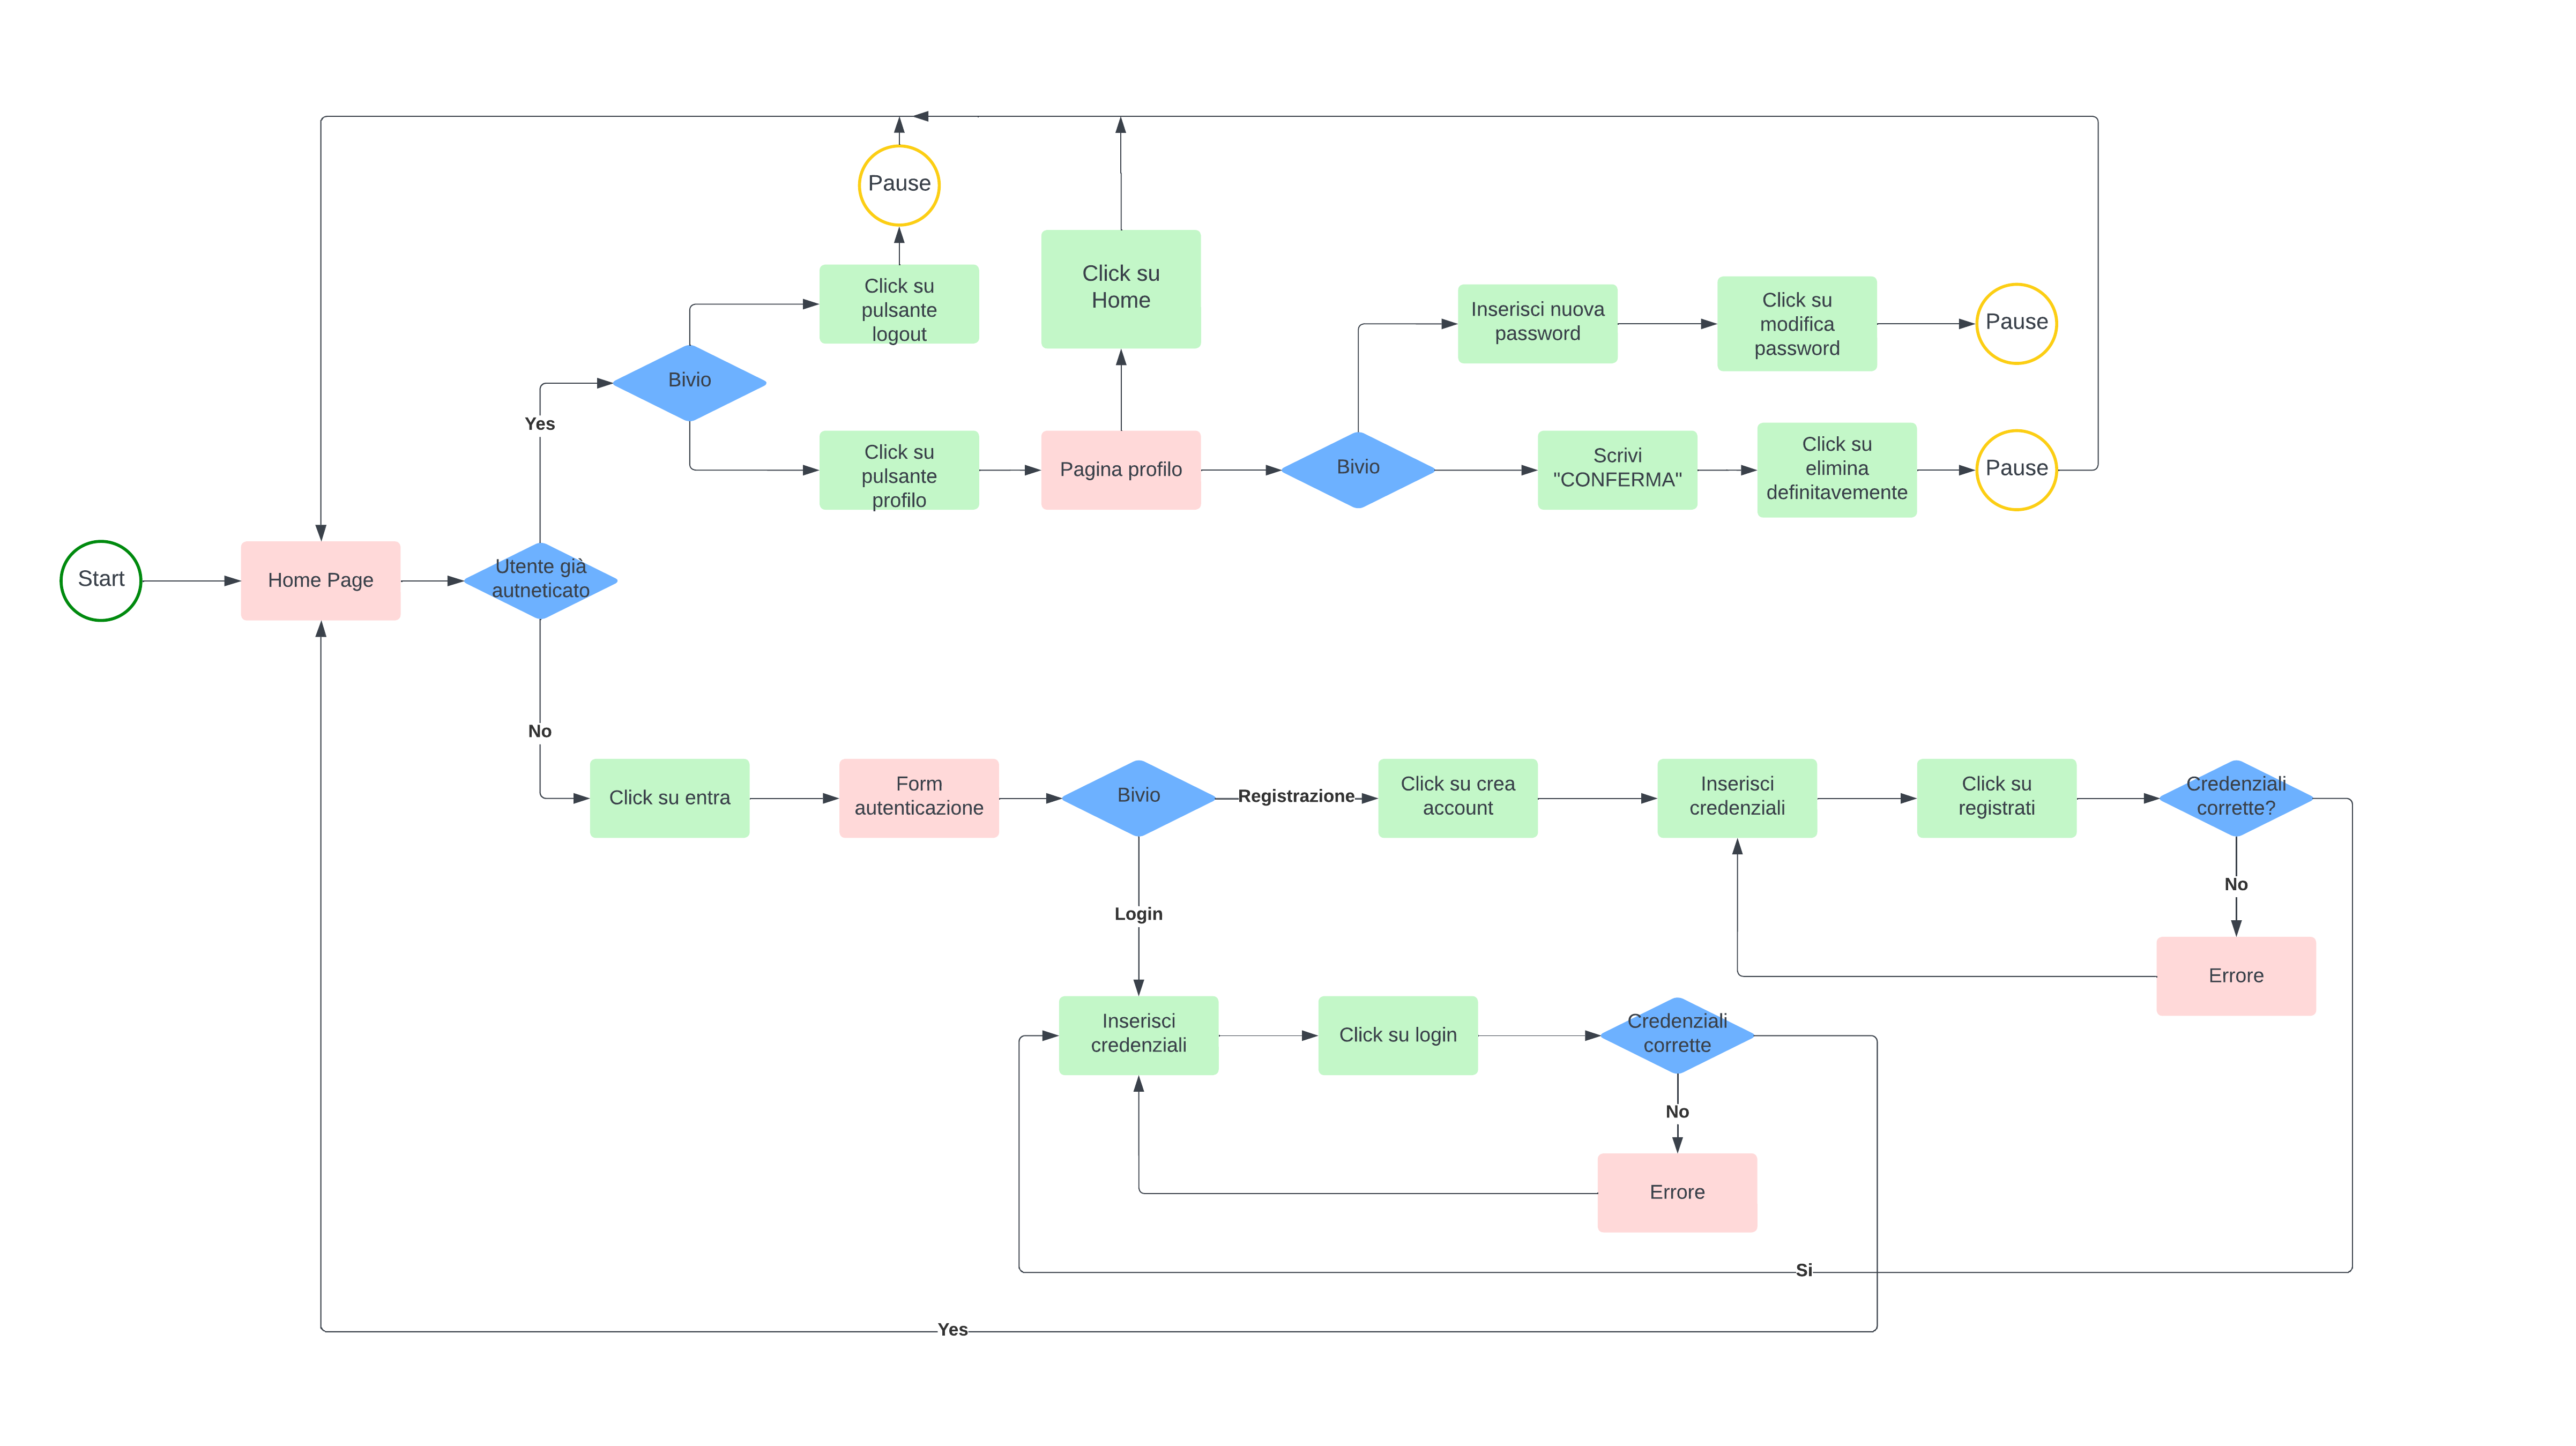
\includegraphics[width=\textwidth]{materiale/UserFlow Autenticazione.png}
\newpage
\subsection{Azioni riguardanti l'utilizzo del sito}
Questo User Flow è specifico per tutte le azioni che ogni tipo di utente può intraprendere nell'utilizzo del sito, teniamo a precisare che la funzione di aggiunta di un problema tramite DB non è stata sviluppata, al momento il form esiste
ma non dialoga col database, ci scusiamo per l'incovenienza. Ricordiamo che tramite Navbar l'utente è in grado di intraprendere tutte le azioni descritte nell'User Flow precedente.

  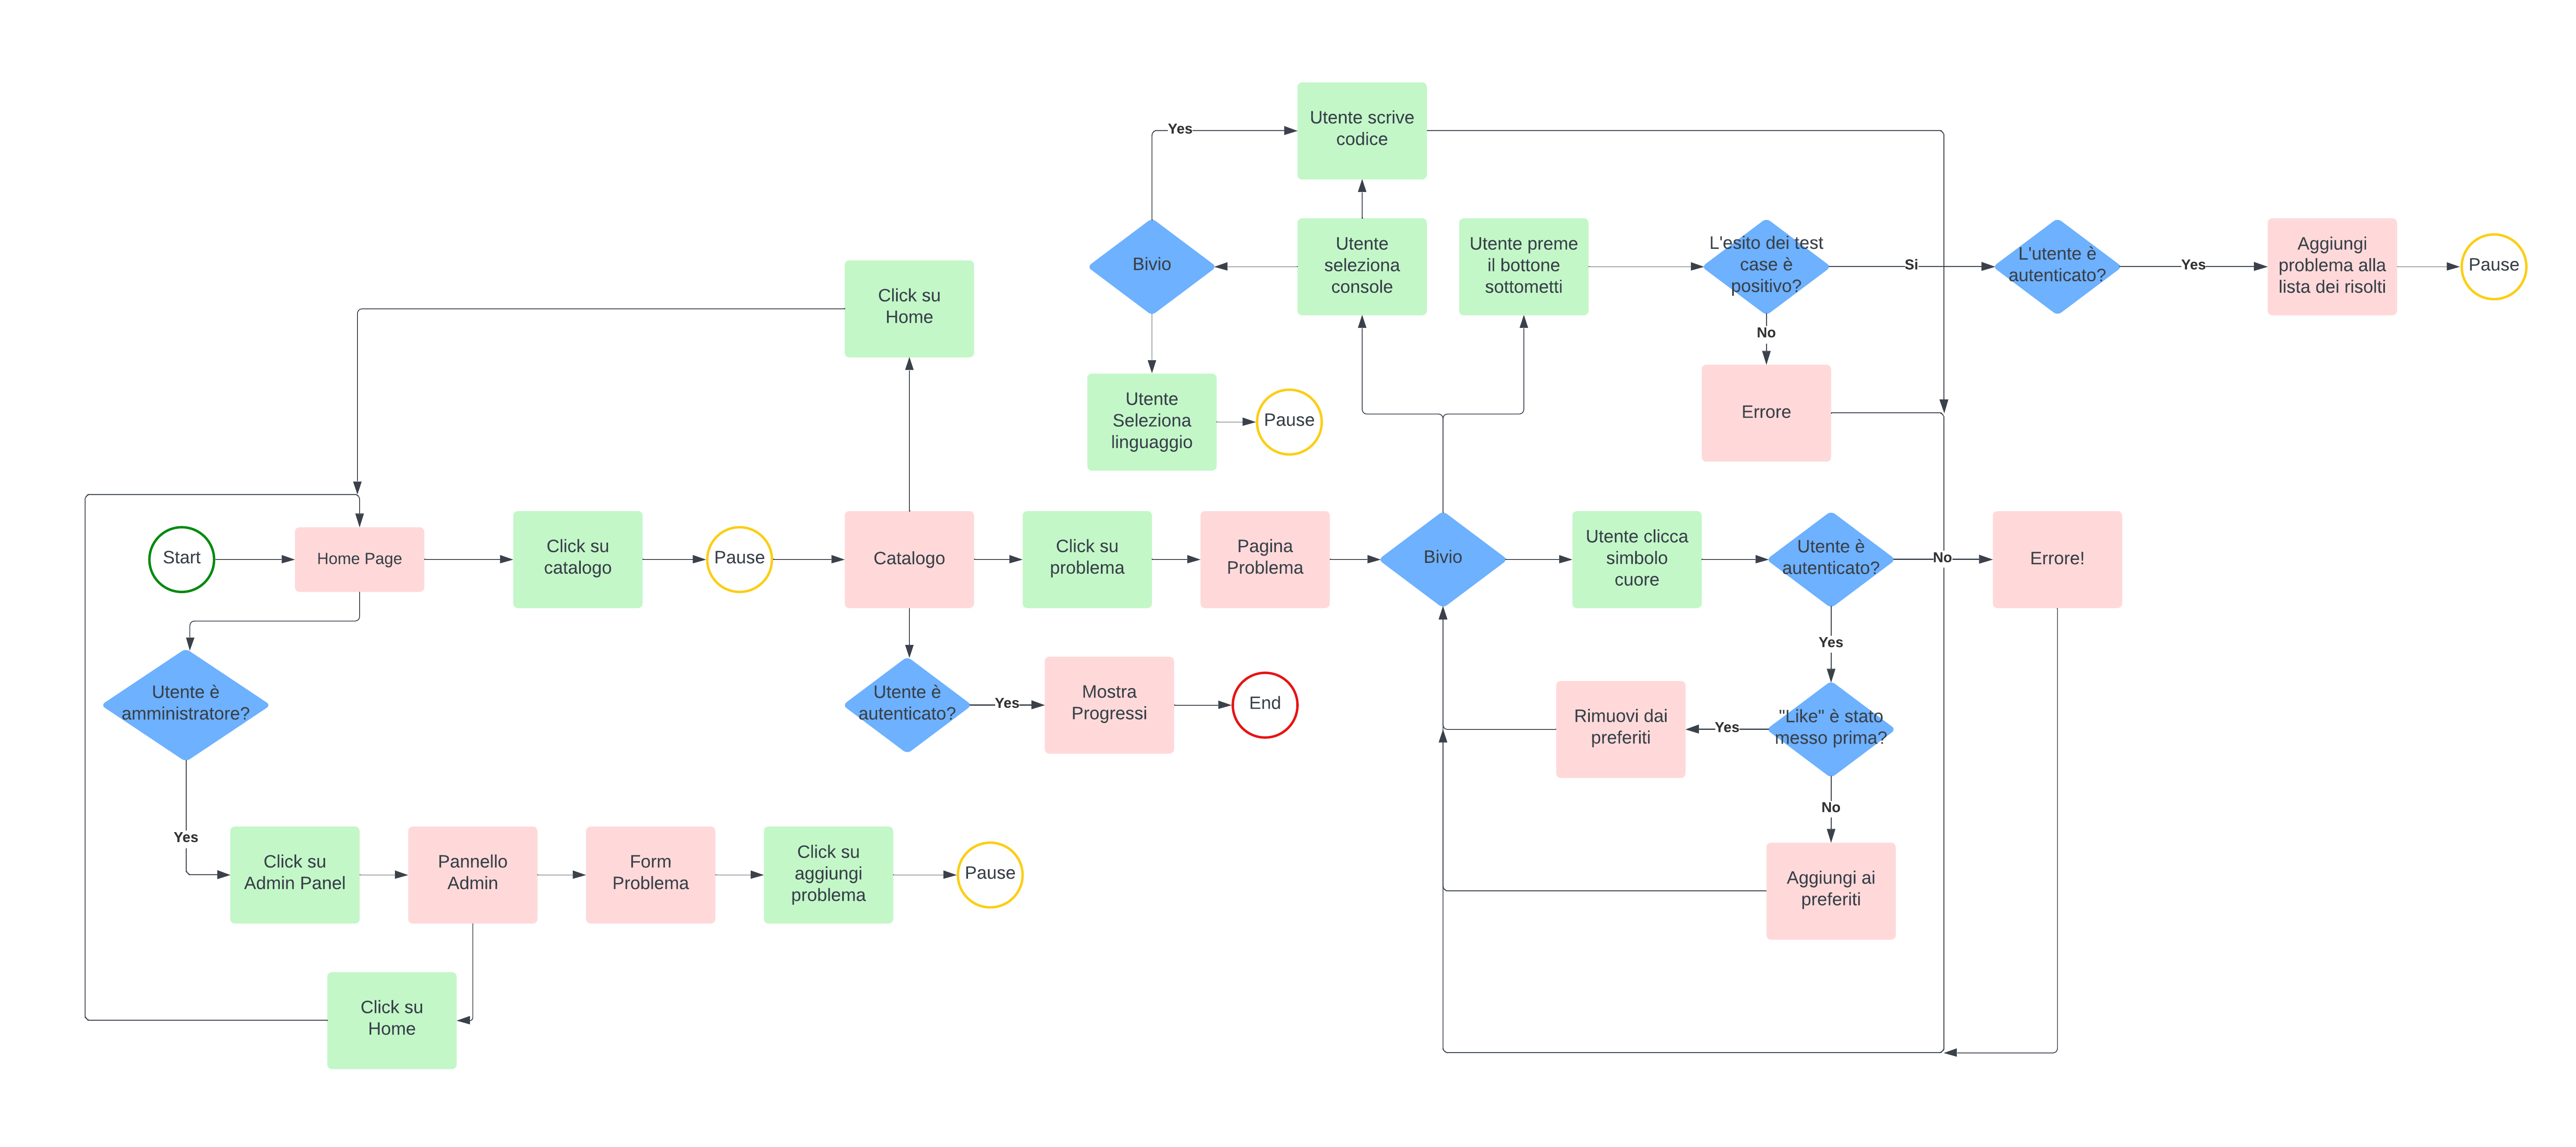
\includegraphics[width=\textwidth]{materiale/UserFlow Utilizzo.png}

\newpage
\section{Documentazione e implementazione dell'applicazione}
Nella precedente sezione abbiamo illustrato tutte le funzioni attualmente implementate nell'applicazione e un'idea di come l'utente può interagire con esse.
L'applicazione \textbf{SleepCode} è stata sviluppata utilizzando \href{https://nextjs.org/}{Next.js} vers. 14.0.3, un framework Javascript free-open source basato su \href{https://react.dev/}{React}
\newpage
\subsection{Struttura del Progetto}
Il software utilizzato per version control utilizzato è \href{https://git-scm.com/}{Git}, come repository abbiamo utilizzato \href{www.github.com}{Github},
il codice e la sua history è presente su una repository del membro del Team Raffaele Castagna, l'ultima versione stabile e quella utilizzata per hostare il sito è disponibile presso la repository CodeBase, all'interno di essa,
troveremo le seguenti cartelle:
\\
\begin{center}
  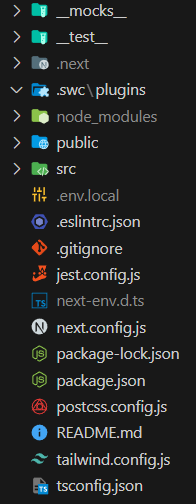
\includegraphics{materiale/Project Structure.png}
\end{center}
Ricordiamo che le cartelle \textbf{.next, .swc, .env} insieme a \textbf{package-lock.json, next-env.d.ts, eslintrc.json} sono state generate automaticamente
\newpage
\subsubsection{Directory: \_\_mock\_\_ }
Questa cartella contine delle funzioni "mock" che permettono a Jest di poter effetuare il testing senza fare chiamate dirette al database.
\subsubsection{Directory: \_\_test\_\_}
Questa cartella contiene tutti i test case e test suite dedicate al testing.
\subsubsection{Directory: public}
Questa cartella contiente tutte le immagini utilizzate all'interno del sito.
\subsubsection{Directory: src}
Questa cartella contiente tutte le parti del progetto sia front-end che back-end del progetto, procediamo con una vista più dettagliata
\begin{center}
  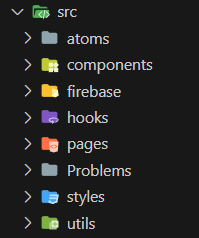
\includegraphics{materiale/src.png}
\end{center}
\begin{itemize}
  \item \textbf{Atoms}: Abbiamo utilizzato una libreria di State management sviluppata da Google per tenere traccia dello stato dell'utente, la libreria utilizzata è: \href{https://recoiljs.org/}{Recoil}, gli atoms non sono altro che gli stati di certi componenti del sito.
  \item \textbf{Components}: Questa cartella contiene tutti i vari componenti del sito che vengono utilizzati dalle pagine, essi possono essere semplici \href{https://www.nngroup.com/articles/skeleton-screens/}{Scheletri} o componenti di maggior importanza.
  \item \textbf{Firebase}: Questa cartella contiene tutti i file relativi al setup di \href{https://firebase.google.com/}{Firebase}, il database utilizzato per il progetto.
  \item \textbf{Hooks}: Questa cartella contiene gli hooks sviluppati durante il progetto per compiere una funzione.
  \item \textbf{Pages}: Questa Cartella contiente le varie pagine le loro \textbf{routes} e le \textbf{API}.
  \item \textbf{Problems}: Questa cartella contiene il tipo di dato generico per i problemi.
  \item \textbf{Styles}: Questa cartella contiene diversi stili pre-impostati utilizzati assieme a \href{https://tailwindcss.com/}{TailwindCSS}
  \item \textbf{Utils}: Questa cartella contiene i diversi testi e informazioni relative ai problemi attualmente disponibili, oltre che a form validators e funzioni comuni.
\end{itemize}
\subsubsection{.env.local}
Questa file contiene tutte le \textbf{variabili locali}, utilizzate per la connessione al database e necessarie per il corretto funzionamento dell'applicativo.
\subsubsection{.gitignore}
Questa cartella specifica quali file \textbf{git} non deve includere nelle varie pull/push requests. (.env.local è più importante in quanto contiente la \textbf{Chiave segreta})
\subsubsection{jest.config.js}
Questo file contiene la configurazione di \textbf{Jest}, libreria utilizzata nel testing.
\subsubsection{package.json}
Questo file contiene le \textbf{dependency} del framework
\subsubsection{README.md}
Questo file contiene informazioni generali sul progetto.
\subsubsection{postcss.config.js}
Questo file è stato auto-generato da \href{https://tailwindcss.com/}{TailwindCSS}
\subsubsection{tailwind.config.js}
Questo file contiene \textbf{pallet} di colori utilizzati da \href{https://tailwindcss.com/}{TailwindCSS}
\subsubsection{tsconfig.json}
Questo file contiene regole utilizzate da \href{https://eslint.org/}{ESLint} un \textbf{patter checker} utilizzato durante lo sviluppo
  
\subsection{Dipendenze del progetto}
Il progetto utilizza diverse librerie, procediamo ad elencarne le più importanti e spiegare il loro funzionamento.
\begin{itemize}
  \item \href{https://codemirror.net/}{\textbf{CodeMirror}}: Utilizzata nel front-end avere uno stile simile a Vs-code durante la scrittura del codice.
  \item \href{https://split.js.org/}{\textbf{Split}}: Utilizzata nel front-end per rendere la pagina dei problemi dinamica (L'utente è in grado di modificare la grandezza dei componenti).
  \item \href{https://www.npmjs.com/package/react-toastify}{\textbf{Toastify}}: Libreria che offre componenti UI utilizzati per dialogare con l'utente.
  \item \href{https://recoiljs.org/}{\textbf{Recoil}}: Libreria di State Management sviluppata da Google.
  \item \href{https://firebase.google.com/docs/build}{\textbf{Librerie fornite da Firebase}}: Abbiamo utilizzato diverse librerie fornite da firebase come \textbf{auth,sdk,admin sdk} e molte altre.
  \item \href{https://www.npmjs.com/package/yup}{\textbf{Yup}}: Utilizzato per la validazione RegEx di dati inseriti
  \item \href{https://eslint.org/}{\textbf{ESLint}}: Pattern checker utilizzato durante lo sviluppo per ottenere un codice di alta qualità
  \item \href{https://jestjs.io/}{\textbf{Jest}}: Libreria utilizzata per il testing
  \item \href{https://www.npmjs.com/package/node-mocks-http}{\textbf{node-mocks-http}}: Libreria utilizzata per mandare richieste API finte durante il testing.
\end{itemize}
Oltre a queste abbia altre dipendenze minore tra vari \textbf{hooks} e pacchetti necessari per altri pacchetti inutili da elencare.
\subsection{Dati del Progetti e Database}

\end{document}